% !TeX root = ../report.tex

\section{Deep Learning}
In this section we will go through an overview of the model used in the "deep learning" attempt at solving the task at hand. The model seeks to solve two subtasks in one go as multi task learning problem. The subtasks are: regression (task 1 in section \ref{sec:task}) and classification (task 5 in section \ref{sec:task}). For task 1 the model also predicts independently of the general emotion felt, i.e. tweets for joy, anger etc. get a 0-to-1 score using the same model.

\subsection{Model overview}

\subsubsection{Preprocessing of text and textual representation} \label{sec:preprop}
For the textual preprocessing, all tweets are read in and converted using a mapping from the word to an integer. This ensures that words get mapped to the same key and also enables an enforcing on the maximum amount of words to be used. Train data is treated differently than development and test data, in that every word read in train data gets converted to a word vector independently based on the word but if an unknown word gets read in the development or test data its numerical value gets replaced by an "unknown" placeholder. One way of countering this is to use pretrained word embeddings. This does not constitute as having read and adapted to the test set, since one could envision having a pretrained word embedding for every word in the entire language.\\
The pretrained embeddings used in the model are retrieved from a large set of pretrained embeddings which have been trained on Twitter data (~400 million tweets). The words in the dataset for the task at hand are then looked up in the pretrained embeddings. If these are not present a zero vector is used instead, which will then be trained from the ground up by the model.\\
Since the model used both word and character representations, the characters were read in separately, although the same basic principle was followed. Every character had a integer mapped to them and this integer would then map to a high dimensional vector with weights that could then be optimized by the network using backpropagation. No pretrained embeddings were used for the characters and so they had to be trained from the ground up, every time.

\subsubsection{Augmentation of data} \label{sec:augm}
The first iteration of the data augmentation consisted of reading in all the data for task 1 and 5 as described in section \ref{sec:preprop}. Since the tweets had different format of truth labels, one was a singular value (regression) and one was a multi-label list (classification), reading in the labels had to be augmented. Since the tweets were reused in the two tasks, some of the regression tweets could be augmented with their respective classification label, although, if no classification label was present the truth labels were set to -1, which would then act as a mask. Since there were more regression tweets than classification, the augmentation was done this way around.\\
All the tweet representations were padded differently based on whether or not the tweet was being read as a word representation or character representation and tweets longer than the specified padding values were cut down to size. 

\subsubsection{Generating pretrained word embeddings}
For the generation of pretrained word embeddings, the twitter Word2Vec model outlined in [GODIN] was used, and 400 dimensional word embeddings were used.\\
KAN IKKE FINDE UD AF OM DET HER CLASHER MED PREPROP SECTIONEN

\subsection{Model output}
Since the model reads in all regression data in one single input and outputs it in a similar bulk manner, the overall feeling from the regression data can not be intrinsically inferred from the regression value, meaning, the way that an "anger tweet" is classified as an anger tweet is its position in the large output matrix. That way, if a completely new tweet would be presented to the model, the value of the regression would be an emotion intensity felt by the tweeter but in a general sense. To help guide the intensity in a direction, the eleven classification labels could be used to infer the tweeters general state of mind. 

\subsection{Loss functions}
Since the model is multi-task model, more than one loss function was needed. The model solves two task which can not share loss functions, the regression and the classification of tweets.

\subsubsection{Regression loss function and metric}
For the regression output of the model, mean squared error was chosen as a way to optimize the model with regards to Pearson-score. Mean squared error is used in the following form:\\
\begin{equation} \label{eq:lreg}
L_{reg}(gold, pred)=\dfrac{1}{b_{size}}\sum^{b_{size}}_{i=1}\left(gold_{i}-pred_{i}\right)^{2}
\end{equation}\\
The Pearson correlation coefficient is calculated thus in the evaluation of the scores:\\
\begin{equation} \label{eq:pearson}
r_{p} = \dfrac{\sum \left(gold-m_{gold}\right) \left(pred-m_{pred}\right)}{\sqrt{\sum \left(gold-m_{gold}\right)^{2} \left(pred-m_{pred}\right)^{2}}},
\end{equation}\\
where \textit{gold} is the truth/gold labels and \textit{pred} is the predictions and \textit{m} is the mean of the vectors subscripted.\\
There are two aspects to getting a good correlation score, i.e. a score of one. This is done by having predictions close to the gold score but also having a mean prediction similar to the gold scores. Getting a mean prediction similar to the mean gold does not necessarily coincide with having similar values. Both of these features will get reduced the closer the prediction values get to the gold values, and therefore the mean squared error proved useful in solving the specific task.\\
\\
The metric used for the regression is mean absolute error:\\
\begin{equation} \label{eq:meanabs}
m_{reg}=\dfrac{1}{b_{size}}\sum^{b_{size}}_{i=1}abs\left(gold_{i}-pred_{i}\right)
\end{equation}\\
Where $b_{size}$ is the batch size used by the model during training. 

\subsubsection{Classification loss function and metric}
The loss function for the classification is a bit more convoluted since all regression tweets have regression labels but not all regression tweets have classification labels. This is handled by way of a mask and the augmentation specified in section \ref{sec:augm}. The loss function is described as such:\\
\begin{equation} \label{eq:fclass}
f(gold,pred) =
     \begin{cases}
       0, &\quad\text{if gold = mask}\\
       wbce(gold,pred), &\quad\text{otherwise} \\
     \end{cases}
\end{equation}\\
where \textit{wbce} is our custom weighted binary cross entropy function. Since the model has eleven output layers, there is a loss function for each of the eleven emotions/layers. The function (\ref{eq:fclass}) is used in a batch wise manner as in the regression case on each emotion:\\
\begin{equation} \label{eq:lemotion}
L_{emotion}=\dfrac{1}{b_{size}} \sum_{i=1}^{b_{size}} f(gold_i, pred_i)
\end{equation}\\
 This loss function ensures that tweets with no classification labels do not impact the updating of the weights of the model by giving the predicted values a loss of zero.\\
Binary cross entropy is defined as follows:\\
\begin{equation}
BCE(gold,pred) = -(gold \cdot log(pred)+(1-gold) \cdot log(1-pred))
\end{equation}\\
The custom weighted binary cross entropy function is defined as follows:\\
\begin{equation}
wBCE(gold,pred) = (gold \cdot 1_{weight} + (1-gold) \cdot 0_{weight}) \cdot BCE(gold, pred)
\end{equation}\\
where $1_{weight}$ and $0_{weight}$ are parameters that can be tuned in the model. This weighting parameter is included because of the uneven distribution of ones and zeros. The goal of the model is to detect whenever emotions are felt by the tweeter, and as such ones are to be valued more if guessed.  \\ \\
The metric used for classification is a custom metric function which builds on binary accuracy. The custom part consists of masking the -1's the same way as the loss function, so that the metric returns a value corresponding to a correct guess whenever classification labels are missing. The custom metric function looks like this: \\
\begin{equation}
f(gold,pred) =
     \begin{cases}
       1, &\quad\text{if gold = mask}\\
       BA(gold,pred), &\quad\text{otherwise} \\
     \end{cases}
\end{equation}\\
where \textit{BA} is defined as follows: \\
\begin{equation} \label{eq:bin_acc}
BA(gold, pred) =
	\begin{cases}
		1, &\quad\text{if gold = round(pred)} \\
		0 &\quad\text{otherwise} \\
	\end{cases}
\end{equation}\\
where the \textit{pred} value is rounded to 0 or 1 since it is a probability value of the guessed emotion.\\
This equation is then used and averaged batch-wise like the loss: \\
\begin{equation} \label{eq:class_metric}
m_{class}=\dfrac{1}{b_{size}}\sum^{b_{size}}_{i=1}f\left(gold_{i}-pred_{i}\right)
\end{equation}\\

\subsubsection{Combined loss function}
The model is trained using the sum of equation (\ref{eq:lreg}) and (\ref{eq:lemotion}):\\
\begin{equation}
L_{combined}(gold,pred)=L_{ratio}\cdot L_{reg}(gold, pred) +  \sum_{e\in E}\dfrac{(1-L_{ratio})}{|E|}\cdot L_{e}(gold, pred),
\end{equation}\\
where \textit{e} is one of the eleven emotions in \textit{E}. The ratio $L_{ratio}$ is a parameter that can be tweaked and can be used to force the model implicitly to weight one task higher than the other. Furthermore, the weighting of the single classification emotions can also be tweaked and given more weighting the others.

\subsection{Model architecture}
Since the model consists of two inputs, character and word representation of the tweets, two separate submodels work in tandem to process the tweets, and the result of these submodels are concatenated after the fact.

DE ER FUCKING LORT DE HER AFSNIT, SKRIV OM

\subsubsection{Word input model}
The word input of the tweets are 60(MAXSENTLEN) $\cdot$ 400(WORDEMBEDDIM) dimensional vectors that have been passed through the preprocessing and augmentation mentioned in section \ref{sec:preprop} and \ref{sec:augm}. These vectors are then passed into two 250-dimensional, bidirectional gated recurrent unit (BRUG GRU?) which traverse the tweet front to back and vice versa, and the outputs of the two GRU layers are then concatenated. This is the output of the word submodel.

\subsubsection{Character input model}
The character input gets processed more than the word inputs. The character input of the tweets are 256(MAXWORDLEN) $\cdot$ 400(CHARDIM) dimensional vectors and these vector get passed into a residual neural network where the vectors get batch normalized. An activation is then applied and 1 dimensional convolution is then applied. This is done twice, and the result of this then fed to a maxpooling layer and added to the input of the residual part of the model. The amount of residual layers is a hyperparameter to be passed to the model. A number of batch normalizations, activation and

\begin{figure}[H]
    \centering
        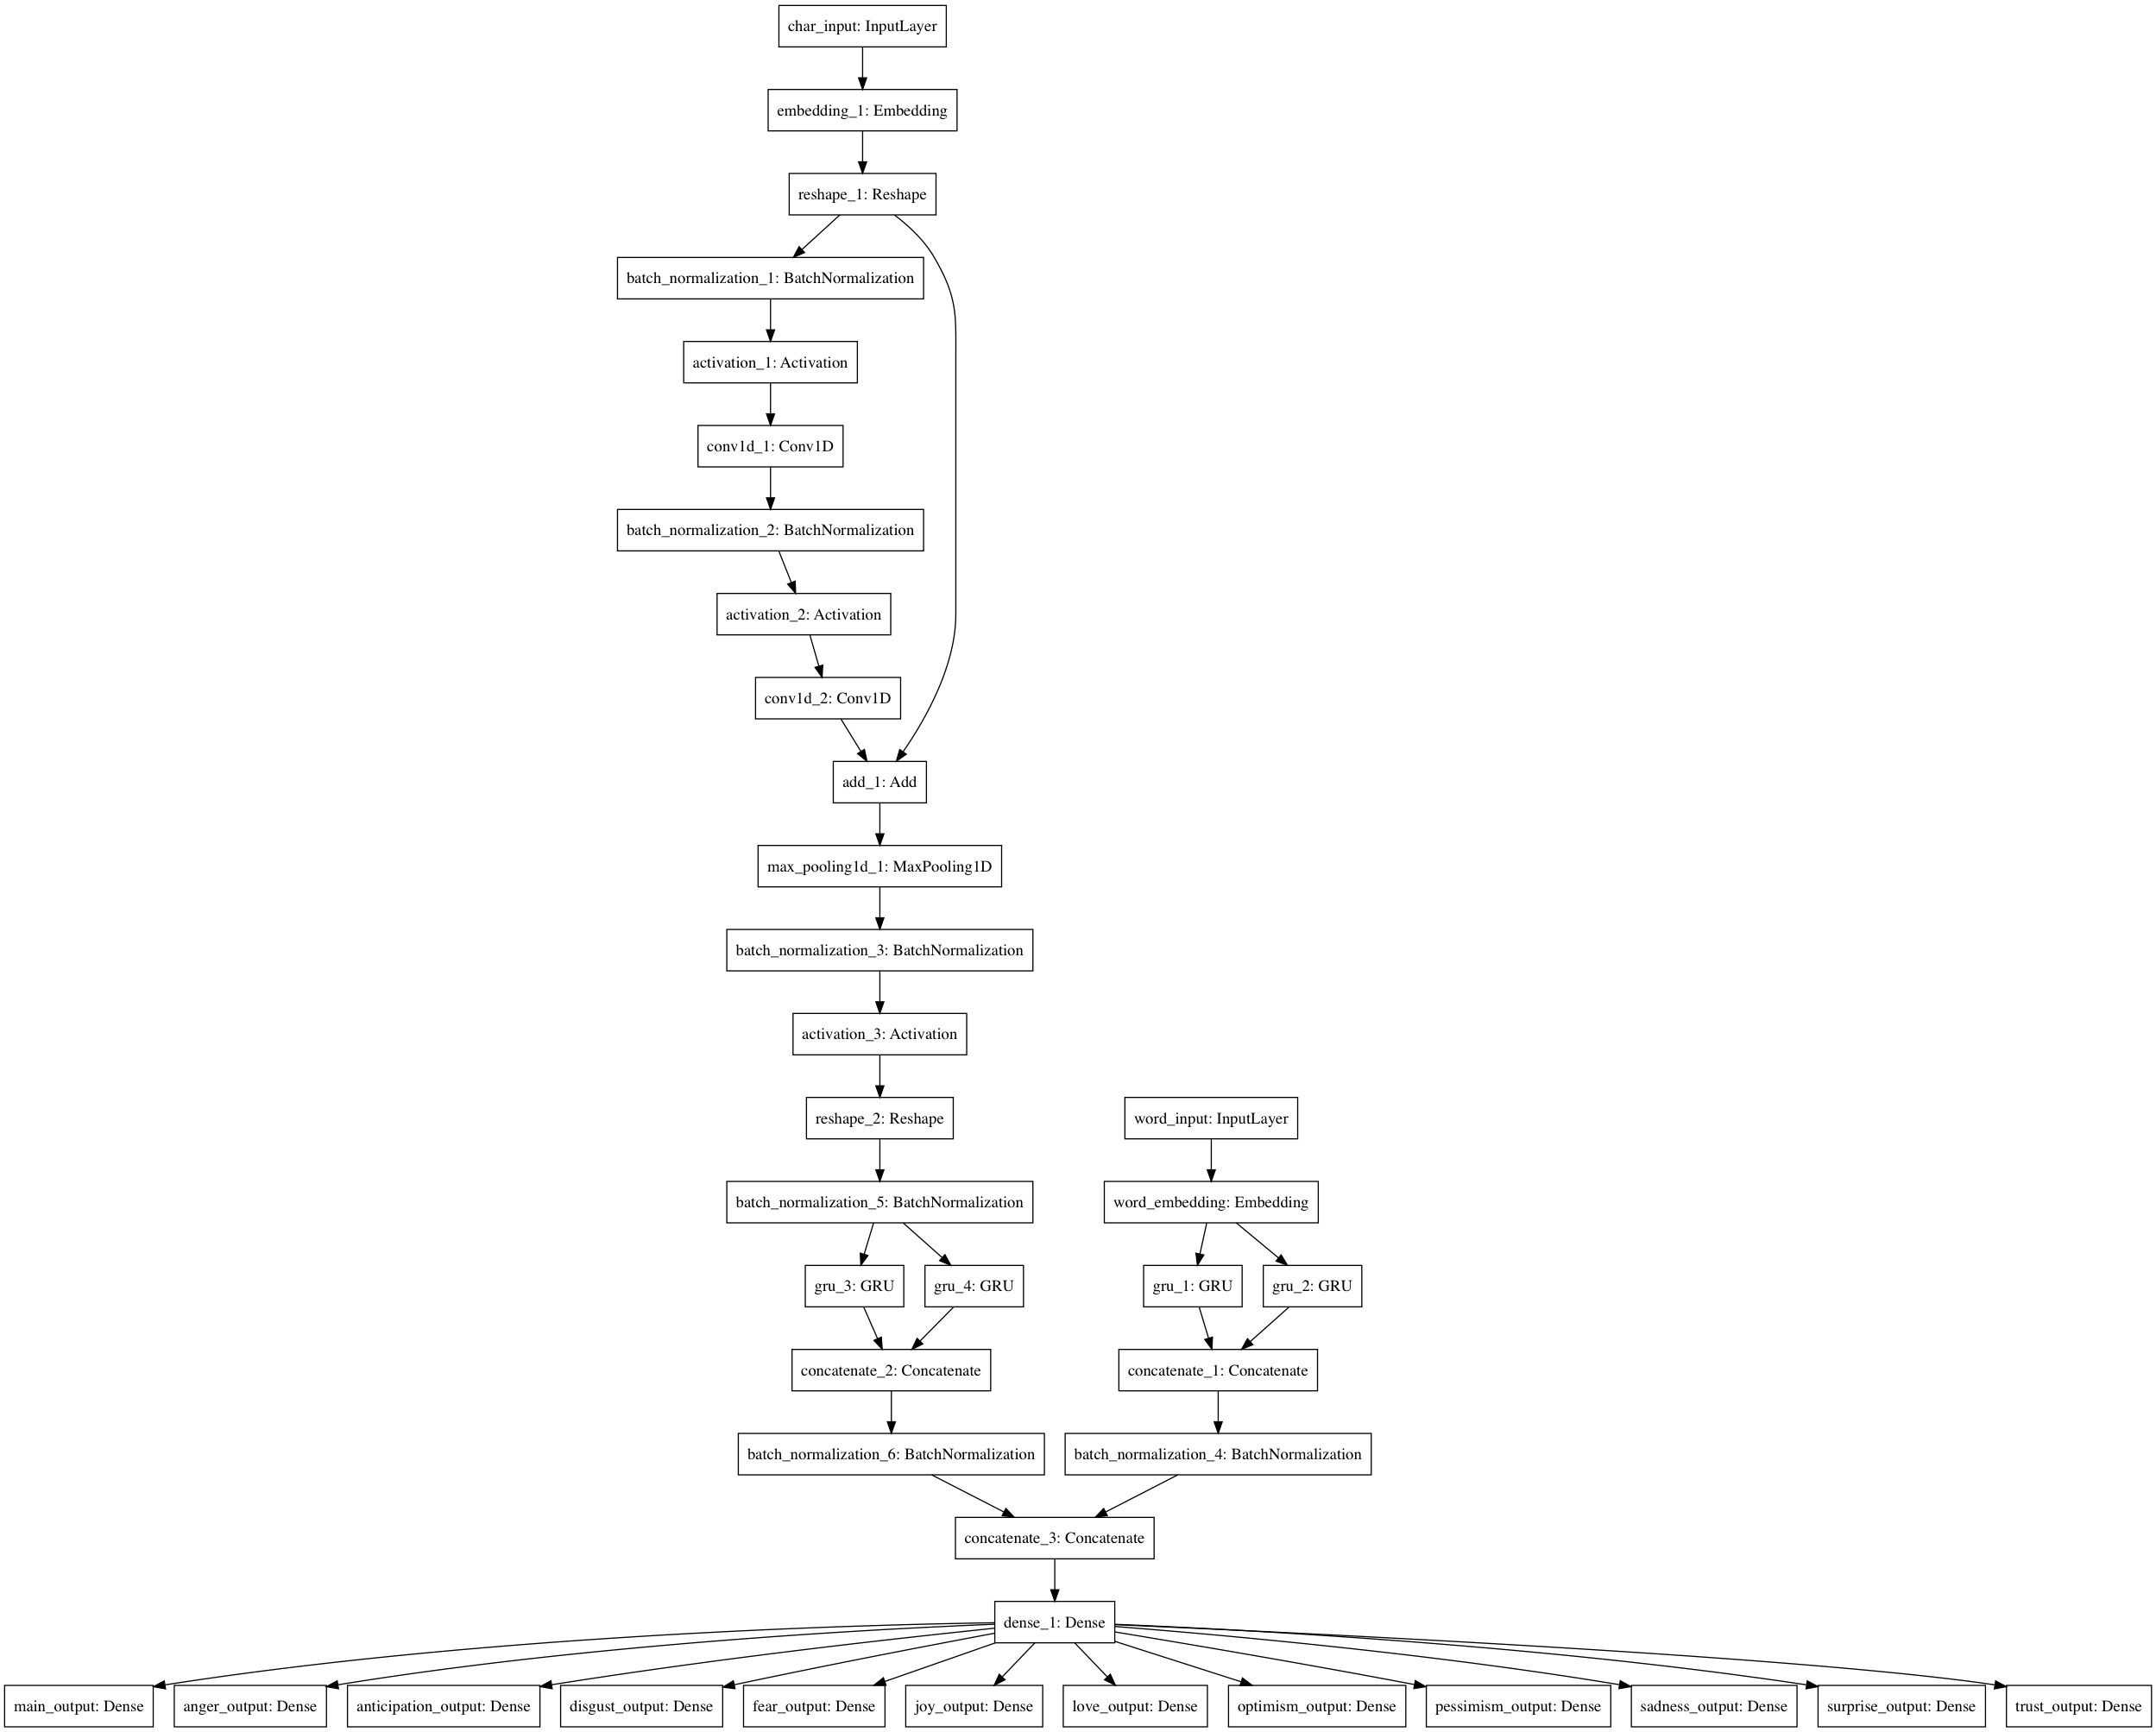
\includegraphics[width=\textwidth]{pictures/model.png}
        \caption{The full model, training on both word and character representations}
        \label{fig:fullmodel}
\end{figure}

\subsection{Results and data}
davdav